% !TEX encoding = UTF-8 Unicode
% ÄÖÜ ß äöü

%The aim of this project was to design an interactive environment on a tablet computer 
%that allows the user to learn simple facts about the formalism of propositional logic 
%and standard transformations of Boolean functions. 
%The environment was meant to be self-explanatory. 

The core of this concept builds on tutorials with exercises 
and a playground where the %learned 
acquired knowledge can be used in different modes. 
A glossary of terms and a formula calculator to check formulas will support the user in her learning.

\section{Tutorials}

\Nyaya for iPad covers syntax and semantics of propositional logic, 
but only some basic equivalences.
It introduces normal forms, truth tables and binary decision diagrams 
as different but equivalent representations of Boolean functions.

The structure of the tutorials and the content of the exercises are heavily based on %the according
related sections of the book  
{\em Logic in Computer Science}  by M.~Huth and M.~Ryan. \cite{Huth:2004:LCS:975331}
Additional content was taken from the lecture {\em Logic}  by {A. Middeldorp}. \cite{Middeldorp:2012:LICS}


\begin{table}[htdp]
\begin{center}
\begin{lstlisting}[mathescape,firstnumber=5]
  <array> 		<!-- root with title and sections -->
    <string>Tutorials</string> 					<!-- title -->
    <array>			<!-- section with section title and tutorials-->
      <string>Introduction</string> 				<!-- section title -->
      <array>		<!-- tutorial with title and id -->
        <string>Motivation</string> 	<!-- tutorial title -->
        <string>11</string> 						<!-- tutorial id -->
      </array>
		$\square$
\end{lstlisting}
\caption{Tutorials.plist – the configuration file for all tutorials}
\label{tab:TUTORIALPLIST}
\end{center}
\end{table}%

General and specific configurations for the tutorials and additional content for the exercises 
are stored in simple property lists (see \tabref{tab:PLISTDTD}) %\footnote{
%\href{http://www.apple.com/DTDs/PropertyList-1.0.dtd}{http://www.apple.com/DTDs/PropertyList-1.0.dtd}
%(see \tabref{tab:PLISTDTD}). }, 
which are xml-files with some basic data types for data and collections, 
that can be easily read and interpreted by different programs.
The file “Tutorials.plist” (see \tabref{tab:TUTORIALPLIST}) 
provides the basic data about available tutorial sections and tutorial titles 
to build a navigation menu programmatically.

Every tutorial includes a teaching part with examples (HTML-files in UTF-8 encoding) 
and an interactive knowledge checker with exercises, 
where the user gets immediate feedback. 
Every interactive part will present some instructions to master the task.

\subsection{Introduction}

The first tutorial section with four tutorials gives an informal introduction to modeling, 
i.e.\ the translation from sentences in natural language to sentences in the formal language of propositional logic.
Three of the four tutorials
% \hyperref[tut:11]{\textnumero 11}, 
% \hyperref[tut:12]{\textnumero 12}, and
% \hyperref[tut:13]{\textnumero 13} 
use the same content file to present some questions
to check the user's comprehension. 
The fourth tutorial does not include an exercise.

\begin{table}[htdp]
\begin{center}
\begin{lstlisting}[firstnumber=5]
<array>
  <array> 
    <string>If the barometer falls, then it will rain.</string>
    <string>if p then q</string>
    <string>the barometer falls; it will rain</string>
    <string>p $\rightarrow$ q</string>
  </array>
$\square$
\end{lstlisting}
\caption{QA1.plist – content file for the first three tutorials with exercises}
\label{tab:QA1PLIST}
\end{center}
\end{table}%

The content file “QA1.plist” (see \tabref{tab:QA1PLIST}) contains
an array (starts at line 5) 
of arrays of strings that represents sentences and sample solutions for the 
first three exercises.
The first sentence/solutions array of strings starts at line 7 and ends at line 10. 
The first string in the first array (at line 7) is a sentence, 
which must be analyzed in all three exercises. 
The next string (at line 8) is a correct solution for the first exercise,
the third string (at line 9) is a correct solution for the second exercise,
and the last string in the array (at line 10) is a correct solution for the third exercise.  
The next array of strings would start at line 13.

\begin{table}[htdp]
\begin{center}
\begin{lstlisting}[firstnumber=5]
<dict>
  <key>questionLabelText</key>
  <string>Guess the structure …</string>
  <key>answerLabelText</key>
  <string>Use … </string>
   <key>solutionLabelText</key>
   <string>Sample solution</string>
   <key>questionsFile</key>
   <string>QA1</string>
   <key>solutionIndex</key>
   <integer>1</integer>
</dict>
\end{lstlisting}
\caption{11.plist – configuration file for the first exercise}
\label{tab:11PLIST}
\end{center}
\end{table}

Each tutorial has its own configuration file 
(see \tabref{tab:11PLIST})
with a dictionary that
describes the exercise and defines the index of the sample solution,
with which the user's answer will be checked with some tolerance.
The \verb+solutionIndex+ expresses which string 
is to be used as sample solution in the exercise.
The numbers after tutorial titles indicate the position of the tutorials 
and the names of corresponding configuration and content files.
\textnumero 32 represents the 2nd tutorial in the 3rd section and corresponds 
to the tutorial configuration file \verb+32.plist+ and the tutorial content file \verb+tutorial32.html+.

\paragraph{Applications – \textnumero 11.}
\label{tut:11}
{\em{}“The aim of logic in general is to reason about situations.”}\ \cite{Huth:2004:LCS:975331} 
The first tutorial shows, how two different paragraphs in natural language 
can be reduced to the same formal sentence {\em“If p and not q, then r. Not r. p. Therefore, q“}. 
If the reasoning is correct, the user can use it in both situations. 

In the interactive part the user has to ‘guess’ the formal structure of composite sentences in natural language. 
The sentence 
\verb+‘If the barometer falls,+ \verb+then it will rain’+ 
from line 7 of \verb+QA1.plist+ (see \tabref{tab:QA1PLIST})
has to be translated into
\verb+‘if p then q’+ from line 8 (the solution index is defined as 1 in \verb+11.plist+, see \tabref{tab:11PLIST}).

\paragraph{Propositions – \textnumero 12.}
\label{tut:12}

The concept of propositions – simple declarative sentences – 
as indivisible building blocks of propositional logic 
is explained in more detail. Some counter-examples are presented 
and the ambiguity of natural language is demonstrated.

The user has to find the propositions in composite sentences. 
The correct answer for 
\verb+‘If the barometer falls,+ \verb+then it will rain’+ 
would be  
\verb+‘the barometer falls; it will rain’+ 
from line 9 
(the solution index is defined as 2 in \verb+12.plist+).


\paragraph{Connectives – \textnumero 13.}
\label{tut:13}
The basic symbols of propositional logic to connect propositions are introduced. 
The symbols “$\rightarrow$”, “$\neg$”, “$\wedge$”, and “$\vee$”
 will replace “if then”, “not”, “and” and “or”. 

The user hast to find a matching formula in propositional logic.
For the sentence
\verb+‘If the barometer falls,+ \verb+then it will rain’+ 
a correct answer is
\verb+‘p+ $\rightarrow$ \verb+q’+ 
from line 10 
(the solution index is defined as 3 in \verb+13.plist+),
but 
‘$\neg p \vee q$’ would be accepted too.

\paragraph{Limits – \textnumero 14.}
\label{tut:14}
Some examples are given to demonstrate that not every situation can be modeled in propositional logic. 
There is no exercise available for this tutorial.

% The user has to ‘guess’ whether sentences in natural language are suitable for propositional logic.
%\vspace{2cm}
\subsection{Syntax}

After the informal introduction into the atoms and connectives of propositional logic, 
the formal aspects of propositional logic will be introduced to the user.
Again each exercise is configured by a configuration file similar to 
\verb+11.plist+ (see \tabref{tab:11PLIST}),
but without a \verb+questionsFile+ or a \verb+solutionIndex+,
because the content of the syntax exercises will be generated by the app.
The user's solution will be checked without tolerance.

\paragraph{Definition – \textnumero 21.}
\label{tut:21}
The definition of well formed formulas is explained by a strict grammar with mandatory parentheses.

%\begin{table}[htdp]
\begin{center}
\begin{tabular}{rcccccccccc}
$P$	&$::=$	&$p$ 	
	&|		& $(\neg P)$ 
	&|		&  $(P \wedge P)$ 
	&|		&  $(P \vee P)$ 
	&|		&  $(P \rightarrow P)$ \\
\end{tabular}
%\caption{Grammar with mandatory parentheses}
%\label{tab:BNFGRPA}
\end{center}
%\end{table}

The user has to check whether a formula matches this strict definition of 
a propositional formula.
If the formula is well-formed, the user has to write down the name of the root connective, 
i.e.\ negation, conjunction, disjunction or implication. 
If the formula is not well formed, the user has to leave the answer field empty.

\paragraph{Conventions – \textnumero 22.}
\label{tut:22}
The conventions of precedences and associativity  of connectives to save parentheses are introduced. 
The user has to rewrite formulas from strict syntax to formulas using conventions and vice versa.

%\begin{table}[htdp]
\begin{center}
\begin{tabular}{rccclp{1cm}rcccl}
$P$		&$::=$ & $D$ &|& $D \rightarrow P$ 	 \\
$D$		&$::=$ & $C$ &|& $D \vee C$		&& $N$		&$::=$ & $T$ &|& $\neg N$	\\
$C$		&$::=$ & $N$ &|& $C \wedge N$ 	&& $T$		&$::=$ & $p$ &|& $(P)$		\\
\end{tabular}
%\caption{Grammar with precedence and associativity}
%\label{tab:BNFGRPR}
\end{center}
%\end{table}

%\begin{table}[htdp]
%\begin{center}
%\begin{tabular}{rcl}
%P		&$::=$ & D [ $\rightarrow$ P ]\\
%D		&$::=$ & C \{ $\vee$ C \}\\
%C		&$::=$ & N  \{ $\wedge$ N \} \\
%N		&$::=$ & $\neg$N | p | (P) \\
%\end{tabular}
%\caption{EBNF Grammar (with precedences)}
%\label{tab:BNF}
%\end{center}
%\end{table}

\paragraph{Sub-formulas – \textnumero 23.}
\label{tut:23}
Sub-formulas (starting from atoms) are used to build bigger formulas. 
Big formulas are built from many sub-formulas.
In the exercise the user has to extract the set of sub-formulas from composite formulas. 
A correct answer for 
‘$a \vee b \wedge c$’ would be
‘$a,b,c,b\wedge c, a \vee b \wedge c$‘. 
The order of the sub-formulas does not matter and the user can use parentheses as she likes.
But no sub-formula may occur more than once. 
So the answer ‘$c, b\wedge c, b, a \vee b \wedge c, a$‘ would be right too, 
but ‘$a,b,c,b\wedge c, b, a \vee b \wedge c$‘ would be a wrong answer.

\paragraph{Syntax Trees – \textnumero 24.}
\label{tut:24}
Syntax trees  are introduced as graphical representations of well formed formulas. 
The user has to write formulas for presented syntax trees. 
The user can use parentheses as she likes, but still the written formulas have to match the syntax trees exactly. 
The formula ‘$a \vee b$’ does not match the syntax tree representing the formula ‘$b \vee a$’, 
where the atom node ‘$a$’ is on the right branch of the disjunction node ‘$\vee$’,
nor does ‘$a \vee b \vee c$’ match ‘$a \vee (b \vee c)$’.

\paragraph{Top and Bottom – \textnumero 25.}
\label{tut:25}
The symbols “$\top$” (top) and “$ \bot$” (bottom) are defined
as abbreviations of conjunctions and disjunctions 
of formulas with their negation). Additional basic equivalences are introduced.
The user has to simplify given formulas using tautologies, contradictions and basic equivalences.
%\begin{table}[htdp]
\begin{center}
\begin{tabular}{lll}
$P \vee \neg P \equiv \neg P \vee P\equiv \top$  &
$P \wedge \neg P \equiv \neg P \wedge P \equiv  \bot$\\
$P \vee P \equiv P$ &
$P \wedge P \equiv P$\\
$P \vee Q \equiv Q \vee P$ &
$P \wedge Q \equiv Q \wedge P$ &
$\neg \neg P \equiv P$
\end{tabular}
%\caption{tautologies and contradictions}
%\label{tab:TopBottom}
\end{center}
%\end{table}



%\subsubsection{Simplifying formulas – basic natural deduction rules}
%\label{tut:206}

%(206) The tutorial teaches the simplifying of conjunctions and disjunctions with top, bottom and/or the same sub formulas.
%
%
%
%\begin{table}[htdp]
%\begin{center}
%\begin{tabular}{c|c|c|c|c}
%$\neg \neg P$ & $P \vee P$ & $P \wedge P$ & $P \vee Q$ & $P \wedge Q$\\
%\hline
%$P$ & $P$ & $P$ & $Q \vee P$ & $Q \wedge P$\\
%\end{tabular}
%\caption{basic rules}
%\label{tab:BasicRules}
%\end{center}
%\end{table}
%
%The user has to rewrite some formulas eleminating 
%top, bottom, double negations, conjunctions and disjunctions 
%by using rules from 
%\tabref{tab:TopBottom} and \tabref{tab:BasicRules}.

%\subsubsection{Conjunctive Normal Form} 
%\label{tut:207}
%(207) The syntax of formulas in conjunctive normal form is introduced (\tabref{tab:CNF}) and explained.
%It is shown that some formulas in cnf can be simplified to top.

%
%The user has to guess if a presented formula is in conjunctive normal form
%and if it can be simplified to top ($\top$).


%\subsubsection{Disjunctive Normal Form} 
%\label{tut:208}
%(208) The syntax of formulas in disjunctive normal form is introduced (\tabref{tab:DNF}) and explained.
%It is shown that some formulas in dnf can be simplified to bottom.

%
%The user has to guess if a presented formula is in disjunctive normal form
%and if it can be simplified to bottom ($\bot$).


\subsection{Semantics}

After the introduction of well formed formulas the meaning of logical connectives is defined.
Configuration files are used again, the exercise context is generated randomly by the app, 
but exercise \textnumero 33 
also uses a context file with exemplary entailments that would not likely be generated.

\paragraph{Valuation – \textnumero 31.}
\label{tut:31}
The truth assignment for atoms $(p,q,r,…)$ will be introduced. 
The extended valuation for negation, conjunction, disjunction and implication will be defined.
The valuation of arbitrary formulas by evaluating all sub-formulas is described.
The user has to guess or calculate the evaluation of a given formula with a given truth assignment for the atoms of the formula.

\paragraph{Truth Tables – \textnumero 32.}
\label{tut:32}
The concept of truth tables is explained and demonstrated with the basic connectives. 
The valuation of arbitrary formulas by evaluating all sub-formulas is demonstrated again.
The user has to fill in truth tables for formulas with a maximum of three atoms.

\paragraph{Entailment and Equivalence – \textnumero 33.}
\label{tut:33}
Semantic entailment and equivalence is defined and explained with various examples.
The user has to guess or calculate whether a given semantic entailment or equivalence holds. 

\paragraph{Satisfiability and Validity – \textnumero 34.}
\label{tut:34}
The properties satisfiability and validity of propositional formulas are defined and demonstrated. 
The relationship of these properties with top and bottom is mentioned. 
The user has to guess or calculate whether a given formula is satisfiable or valid.

\subsection{Normal Forms}

The advantages of propositional formulas in special shapes will be emphasized.
%\hyperref[tut:207]{CNFs} and \hyperref[tut:208]{DNFs} are already defined
%in \tabref{tab:CNF} and \tabref{tab:DNF}.
The definitions of implication free forms, negation normal form, 
conjunctive normal forms and disjunctive normal forms will be provided. 
A recipe to transform arbitrary propositional formulas into specific normal forms will be delivered.
Rules to detect satisfiability or validity from normal forms will be mentioned.

\subsubsection{Implication Free Form – \textnumero 41.}
\label{tut:41}
By removing the rule $P ::= D \rightarrow P$ in \vref{tut:22} 
and optimizing the resulting grammar
the implication free form is defined for propositional formulas.
The equivalence transformation
for removing implications is presented
and proved with a truth table. 

%\begin{table}[htdp]
\begin{center}
\begin{tabular}{rccclp{1cm}rcccl}
$D$		&$::=$ & $C$ &|& $C \vee D$		&& $N$		&$::=$ & $T$ &|& $\neg N$	\\
$C$		&$::=$ & $N$ &|& $N \wedge C$ 	&& $T$		&$::=$ & $p$ &|& $(D)$	\\
\end{tabular}
%\caption{Grammar without implications}
%\label{tab:BNFGRIFF}
\end{center}
%\end{table}

The user has to check whether a given formula is implication free.
If the formula is not implication free the user has to transform it into an implication free form
using the equivalence transformation.

\begin{table}[htdp]
\begin{center}
%\begin{tabular}{c}
$P \rightarrow Q \equiv \neg P \;\vee\; Q$
%\end{tabular}
%\caption{Equivalence transformation towards implication free form}
%\label{tab:ET_IFF}
\end{center}
\end{table}

\subsubsection{Negation Normal Form – \textnumero 42.}
\label{tut:42}
By removing all rules for arbitrary negations 
and optimizing the resulting grammar, 
the negation normal form is defined  for propositional formulas. 
The equivalence transformations to transform negations of conjunctions,
negations of disjunctions, 
and double negations
into negation normal forms are presented 
and proved with truth tables.

%\begin{table}[htdp]
\begin{center}
\begin{tabular}{rccclp{1cm}rcccc}
$D$		&$::=$ & $C$ 		&|& 	$C \vee D$	&&	$N$		&$::=$ & $(D)$ 	&|& 	$L$\\
$C$		&$::=$ & $N$ 		&|& 	$N \wedge C$ 	&&	$L$		&$::=$ & $p $ 		&|& 	$\neg p$
\end{tabular}
%\caption{Grammar for negation normal form – \textnumero }
%\label{tab:BNFGRNNF}
\end{center}
%\end{table}

The user has to check whether a given formula is in negation normal form.
If the formula is not in negation normal form
the user has to transform it into negation normal form
using the equivalence transformation for implications and the equivalence transformations for negations.
The rule for double negations is already known from \vref{tut:25}.

%\begin{table}[htdp]
\begin{center}
\begin{tabular}{cp{5mm}cp{5mm}c}
$\neg (P \wedge Q) \equiv \neg P \vee \neg Q$& &
$\neg \neg P \equiv P$ & &
$\neg (P \vee Q)  \equiv \neg P \wedge \neg Q$
\end{tabular}
%\caption{Equivalence transformations towards negation normal form}
%\label{tab:ET_NNF}
\end{center}
%\end{table}

\subsubsection{Conjunctive Normal Form – \textnumero 43.}
\label{tut:43}
A formula in conjunctive normal form is a conjunctive concatenation of disjunctive clauses.
A disjunctive clause is a disjunctive concatenation of literals. 
A literal is an atom or the negation of an atom. 
The distributions of disjunctions over conjunctions is presented
and proved with a truth table.

%\begin{table}[htdp]
\begin{center}
\begin{tabular}{rccccp{1cm}rcccl}
$C$	&$::=$ & $(D)$ 	&$|$ & $(D) \wedge C$ \\
$D$	&$::=$ & $L$ 	&$|$ & $L \vee D$ &&
$L$	&$::=$ & $p$ 	&$|$ & $\neg p$ 
\end{tabular}
%\caption{Grammar for conjunctive normal form}
%\label{tab:CNF}
\end{center}
%\end{table}

The user has to rewrite formulas to conjunctive normal forms.  
All presented formulas are in negation normal form 
but may already be in conjunctive normal form.
The user has to apply the distributions of disjunctions over conjunctions 
none, once or multiple times
as equivalence transformations towards conjunctive normal form.

%\begin{table}[htdp]
\begin{center}
\begin{tabular}{cp{5mm}c}
$P \vee (Q \wedge R) \equiv (P\vee Q) \wedge (P\vee R)$ & &
$(P \wedge Q) \vee R \equiv (P\vee R) \wedge (Q\vee R)$
\end{tabular}
%\caption{Equivalence transformations towards conjunctive normal form}
%\label{tab:ET_CNF}
\end{center}
%\end{table}


\subsubsection{Disjunctive Normal Form – \textnumero 44.}
\label{tut:44}
A formula in disjunctive normal form is a disjunctive concatenation of conjunctive clauses.
A conjunctive clause is a conjunctive concatenation of literals. 
A literal is an atom or the negation of an atom. 
The distributions of conjunctions over disjunctions is presented
and proved with truth tables.

%\begin{table}[htdp]
\begin{center}
\begin{tabular}{rccccp{1cm}rcccl}
$D$	&$::=$ & $C$ 	&$|$ & $C \;\vee D$\\
$C$	&$::=$ & $L$ 	&$|$ & $L \wedge C$ &&
$L$	&$::=$ & $p$ 	&$|$ & $\neg p$
\end{tabular}
%\caption{Grammar for disjunctive normal form}
%\label{tab:DNF}
\end{center}
%\end{table}

The user has to rewrite formulas to disjunctive normal forms. 
All presented formulas are in negation normal form 
but may already be in disjunctive normal form.
The user has to apply the distributions of conjunctions over disjunctions 
none, once or multiple times as
equivalence transformations towards disjunctive normal form.


%\begin{table}[htdp]
\begin{center}
\begin{tabular}{cp{5mm}c}
$P \wedge (Q \vee R) \equiv (P\wedge Q) \vee (P\wedge Q)$ 			& &
$(P \wedge Q) \wedge R \equiv (P\wedge R) \vee (Q\wedge R)$
\end{tabular}
%\caption{Equivalence transformations towards disjunctive normal form}
%\label{tab:ET_DNF}
\end{center}
%\end{table}



%\subsubsection{From general formula to CNF or DNF}
%\label{tut:406}
%(406)
%To combination of the previous techniques to reach a equivalent representation in conjunctive or disjunctive normal form is provided.
%The potential exponential growing of the length of these transformations is demonstrated.
%
%The user has to rewrite formulas to a conjunctive or disjunctive normal form.
%The presented formula is in general form
%but may already be in the demanded normal form.
%
%\subsubsection{Validity of CNF}
%\label{tut:407} 
%(407) 
%If every disjunctive clause contains at least two contemplementary literals.
%then a formula in conjunctive normal form  is valid (a tautology).
%
%The user has to guess or calculate satisfiability of formulas in conjunctive normal form.
%
%\subsubsection{Satisfiability of DNF} 
%\label{tut:408}
%(408) 
%If every conjunctive clause contains at least two contemplementary literals,
%then a formula in disjunctive normal form  is not satisfiable (a contradiction).
%
%The user has to to guess or calculate satisfiability of formulas in disjunctive normal form.

\subsection{Binary Decision Diagrams}

The definition of Boolean functions is introduced. 
Propositional formulas and syntax trees from the previous sections are representations of Boolean functions.
Boolean expressions and binary decision diagrams are additional representations of Boolean functions.

\paragraph{Boolean functions - \textnumero 51.}
\label{tut:51}
N-ary Boolean functions are introduced as mapping from n-tupels of 0s and 1s to the set ${0,1}$.
The Boolean operators $\bar{ \;\;}\;+\;\cdot\;\oplus$ are introduced as special representations of
specific unitary and binary Boolean functions. 
For convenience  in the exercises
an exclamation mark $!(B)$ 
will be used for the negation of a Boolean expression $B$ instead of the bar $\bar{B}$. 
The user has to guess or calculate the results for composite expressions.

\paragraph{Boolean expressions - \textnumero 52.}
\label{tut:52}
The grammar for Boolean expressions is defined. 
The equivalence relation of Boolean expressions is explained.

%\begin{table}[htdp]
\begin{center}
\begin{tabular}{rcccccccccc}
$B$	&$::=$	&$p$ 	
	&|		& $(\overline{B})$ 
	&|		&  $(B \cdot B)$ 
	&|		&  $(B + B)$ 
	&|		&  $(B \oplus B)$ \\
\end{tabular}
%\caption{Grammar for Boolean expressions}
%\label{tab:BNFGRBE}
\end{center}
%\end{table}

The user has to rewrite formulas with propositional symbols into Boolean expressions.
The implication may be a challenge for some users, 
but is doable because the implication free form was introduced 
in an earlier tutorial.

\paragraph{Binary Decisions - \textnumero 53.}
\label{tut:53}
Binary decision nodes are introduced. 
The valuation of binary decision trees is explained.
The user has to fill in the result nodes in a binary decision tree for a given Boolean expression.

\paragraph{Binary Decision Diagrams - \textnumero 54.}
\label{tut:54}
Arbitrary binary decision diagrams are explained. 
Ordered and reduced binary decision diagrams are introduced.
%The user has to check whether a binary decision diagram is ordered and/or reduced.
There is no exercise available for this tutorial.

\newpage
\section{Playground}

On the playground the user can create arbitrary propositional formulas 
by building syntax trees interactively.
Truth assignments can be applied and will be visualized.
The playground supports two modes for working with a syntax tree.

\subsection{Free mode} 

In the free mode an arbitrary formula can be manipulated 
by adding, replacing and removing connectives and atoms. 
The process starts with an atom, which can be expanded or replaced. 
Connectives can be changed at any time, and sub-formulas can be reordered.
The smallest possible formula consists of one atom with a symbol from the set 
$\{ \top, \bot, p, q, r, ... \}$.

Truth values can be assigned to leaf nodes, 
which represent the atoms of the corresponding propositional formula. 
By default no truth values are assigned to atoms, which is visualized by a blue color of the node.
A green color represents ‘true’, and a red color ‘false’.
The valuation of connective nodes is calculated automatically 
and displayed using the same blue, green and red colors.

\subsection{Locked mode}

In the locked mode only equivalence transformations (see \tabref{tab:ET:ALL})
can be applied to nodes of a syntax tree.
The offered transformations depend on the type of node selected by the user. 

In the locked mode the valuation of atoms can not be changed, 
but the automatic valuation of sub-formulas is still active.
The user can observe that equivalence transformations do no change the valuation of the root node.


\subsection{Remarks}

Connective nodes of obvious tautologies like
$P \vee \neg P$ or
$P \rightarrow P$ are displayed with a green color – 
independent from the valuation status of any sub-node.

Connective nodes of obvious contradictions like $P \wedge \neg P$ are displayed with a red color – 
independent from the valuation status of any sub-node.

While working with a syntax tree, the corresponding propositional formula is shown on top of the playground.

While selecting a sub-node of the syntax tree – the root of a sub-tree – 
for manipulation the corresponding sub-formula will be highlighted in the corresponding propositional formula.


\begin{table}[htdp]
\begin{center}
\begin{tabular}{rcl|rcl}

$P$&$ \TAP{\rightarrow}$&$Q$				&$ $&$\TAP{\neg}$&$\neg P$			\\
\hline
$\neg P $&$ \TAP{\vee}$&$Q$					&$ $&$\TAP{P}$&$ $				\\
\\
$ $&$\TAP{\neg}$&$(P \vee Q)$				&$ $&$ \TAP{\neg}$&$(P \wedge Q)$	\\
\hline
$\neg P$&$\TAP{\wedge}$&$\neg Q$			&$\neg P$&$ \TAP{\vee}$&$\neg Q$	\\
\\
$P$&$\TAP{\vee}$&$P$						&$P$&$ \TAP{\wedge}$&$P$			\\
\hline
$$&$\TAP{P}$&$$							&$$&$ \TAP{P}$&$$					\\
\\
$P$&$\TAP{\vee}$&$\neg P$					&P&$\TAP{\wedge}$&$\neg P$		\\
\hline
$ $&$\TAP{\top}$&$ 	$						&	&$\TAP{\bot}$&$ $				\\
\\
$P$&$\TAP{\vee}$&$\top$					&P	&$\TAP{\wedge}$&$\top$			\\
\hline
$ $&$\TAP{\top}$&$ 	$						&	&$\TAP{P}$&$ $				\\
\\
$P$&$\TAP{\vee}$&$\bot$					&$P$&$ \TAP{\wedge}$&$\bot$		\\
\hline
$ $&$\TAP{P}$&$ $							&$ $&$ \TAP{\bot}$&$ $				\\
\\
$P$&$\TAP{\vee}$&$Q$						&$P$&$ \TAP{\wedge}$&$Q$			\\
\hline
$Q$&$\TAP{\vee}$&$P$						&$Q$&$ \TAP{\wedge}$&$P$			\\
\\
$P$&$\TAP{\vee}$&$(Q\wedge R)$				&$P$&$\TAP{\wedge}$&$(Q\vee R)$			\\
\hline
$(P\vee Q)$&$\TAP{\wedge}$&$(P\vee R)$		&$(P\wedge Q)$&$\TAP{\vee}$&$(P\wedge R)$	\\
\\
$(P\wedge Q)$&$\TAP{\vee}$&$R$				&$(P\vee Q)$&$\TAP{\wedge}$&$R$			\\
\hline
$(P\vee R)$&$\TAP{\wedge}$&$(Q\vee R)$		&$(P\wedge R)$&$\TAP{\vee}$&$(Q\wedge R)$	\\
\\
$P$&$\TAP{\vee}$&$(Q\vee R)$				&$P$&$\TAP{\wedge}$&$(Q\wedge R)$			\\
\hline
$(P\vee Q)$&$\TAP{\vee}$&$R$			&$(P\wedge Q)$&$\TAP{\wedge}$&$R$		\\
\\
$P$&$ \TAP{\leftrightarrow}$&$Q$					&$P$&$ \TAP{\veebar}$&$Q$			\\
\hline
$P \rightarrow Q $&$ \TAP{\wedge}$&$Q \rightarrow P$	&$\neg(P \rightarrow Q) $&$ \TAP{\vee}$&$\neg (Q \rightarrow P)$

\end{tabular}
\caption{Available equivalence transformations in locked mode}
\label{tab:ET:ALL}
\end{center}
\end{table}

\section{Glossary}

Terms, definitions and truth tables from the tutorials are listed 
an additional content is defined in the glossary.


\section{BoolTool}

The interactive environment contains the functionality of the
web front end of \texttt{BoolTool}\footnote{
\href{http://cl-informatik.uibk.ac.at/software/booltool/}{cl-informatik.uibk.ac.at/software/booltool}}
developed and provided by the Computational Logic research group
of the Institute of Computer Science at the University of Innsbruck.
\Nyaya's reimplementation is referenced as \BoolTool in this document.

\subsection{Input}

\BoolTool supports Latin letters as identifiers for atoms. 
It reads the symbols
\verb#T# as top, 
\verb#F# as bottom,
\verb#!# as negation operator, 
\verb#&# as conjunction operator,
\verb#+# as disjunction operator,
\verb#># as implication operator, 
\verb#^# as exclusive disjunction operator,
and \verb#(# and \verb#)# as parentheses.
These ASCII-symbols can be found on almost every keyboard.
Thereby any formula of propositional logic can be created completely
using only a keyboard attached to an iPad running \Nyaya.

\BoolTool also accepts standard 
and additional symbols of propositional logic and Boolean expressions
(see Appendix \vref{app:SYMBOLS} for a complete list of accepted ASCII characters and symbols),
which are provided by extended and customized on-screen keyboards.
\BoolTool does not limit identifiers to Latin characters, since, for example, 
Chinese symbols are meaningful names for atoms (see \figref{fig:BoolToolChineseInput}).

\begin{figure}[htbp]
\begin{center}
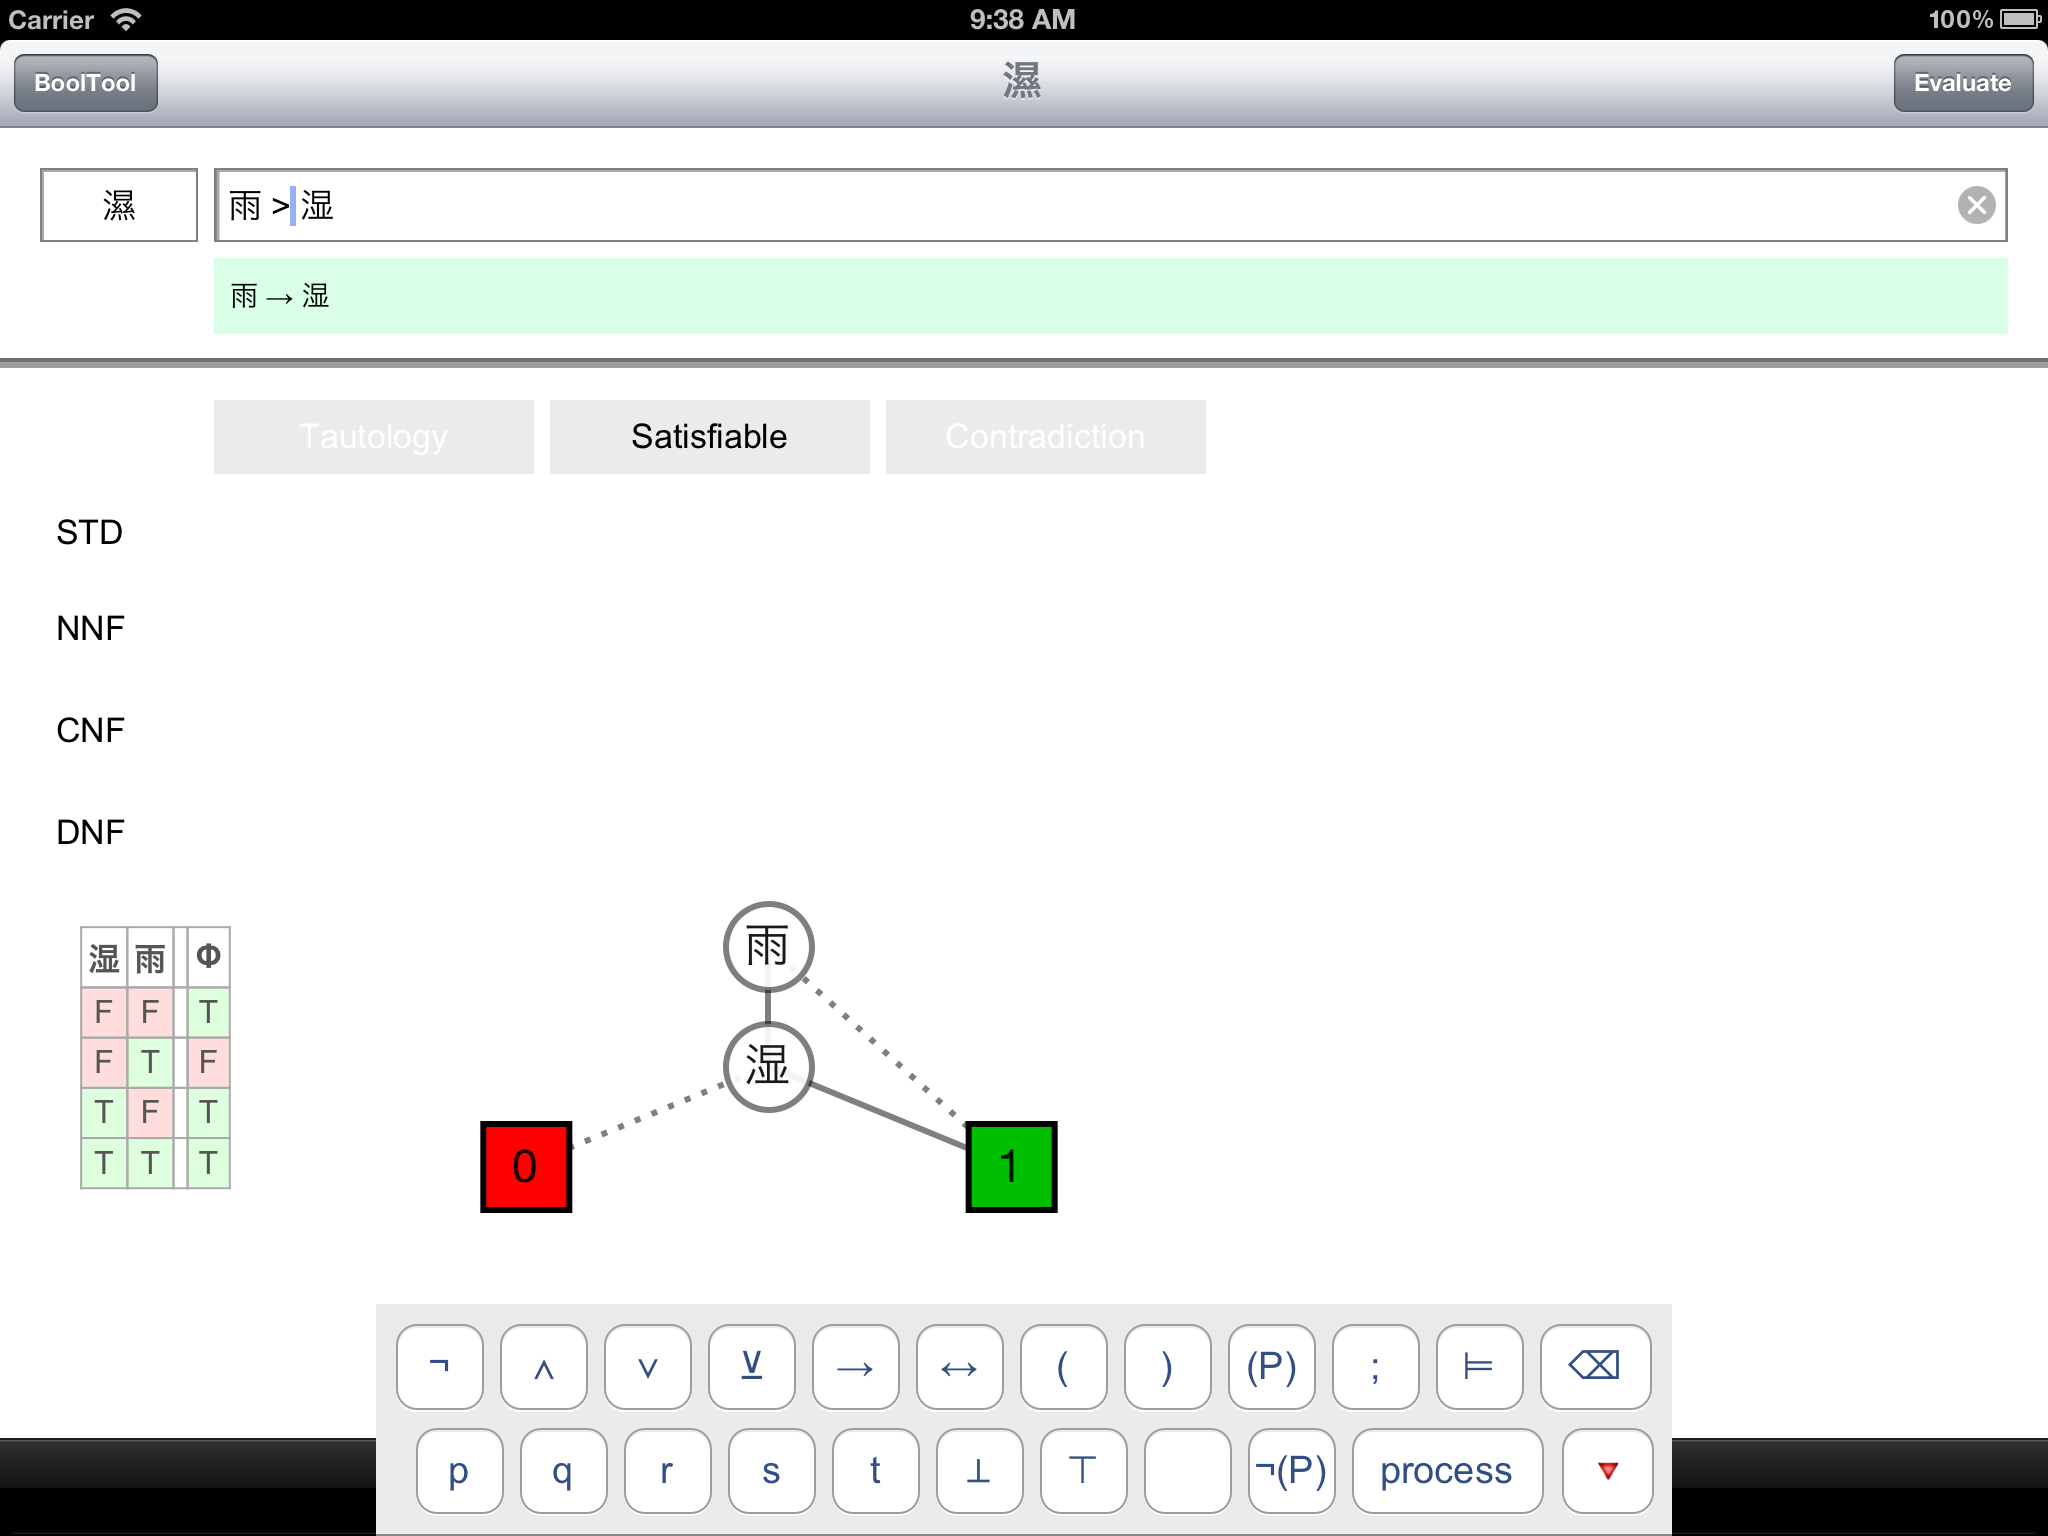
\includegraphics[scale=0.18,trim=0 43cm 0cm 0, clip=true]{concept/RainHD.png}
\caption{Implication with Chinese symbols for rain and wet}
\label{fig:BoolToolChineseInput}
\end{center}
\end{figure}

% ⊨|⊤|⊥|¬|!|∧|&|\\.|∨|\\+|\\||=|↔|<>|→|>|⊻|⊕|\\^|\\(|\\)|,|;|\\w+

\subsection{Output}

\BoolTool calculates validity and satisfiability, 
a conjunctive normal form, 
a disjunctive normal form, 
the truth table and a ordered and
reduced binary decision diagram 
(see \figref{fig:BoolToolROBDD}) of the user's input . 

\begin{figure}[htbp]
\begin{center}
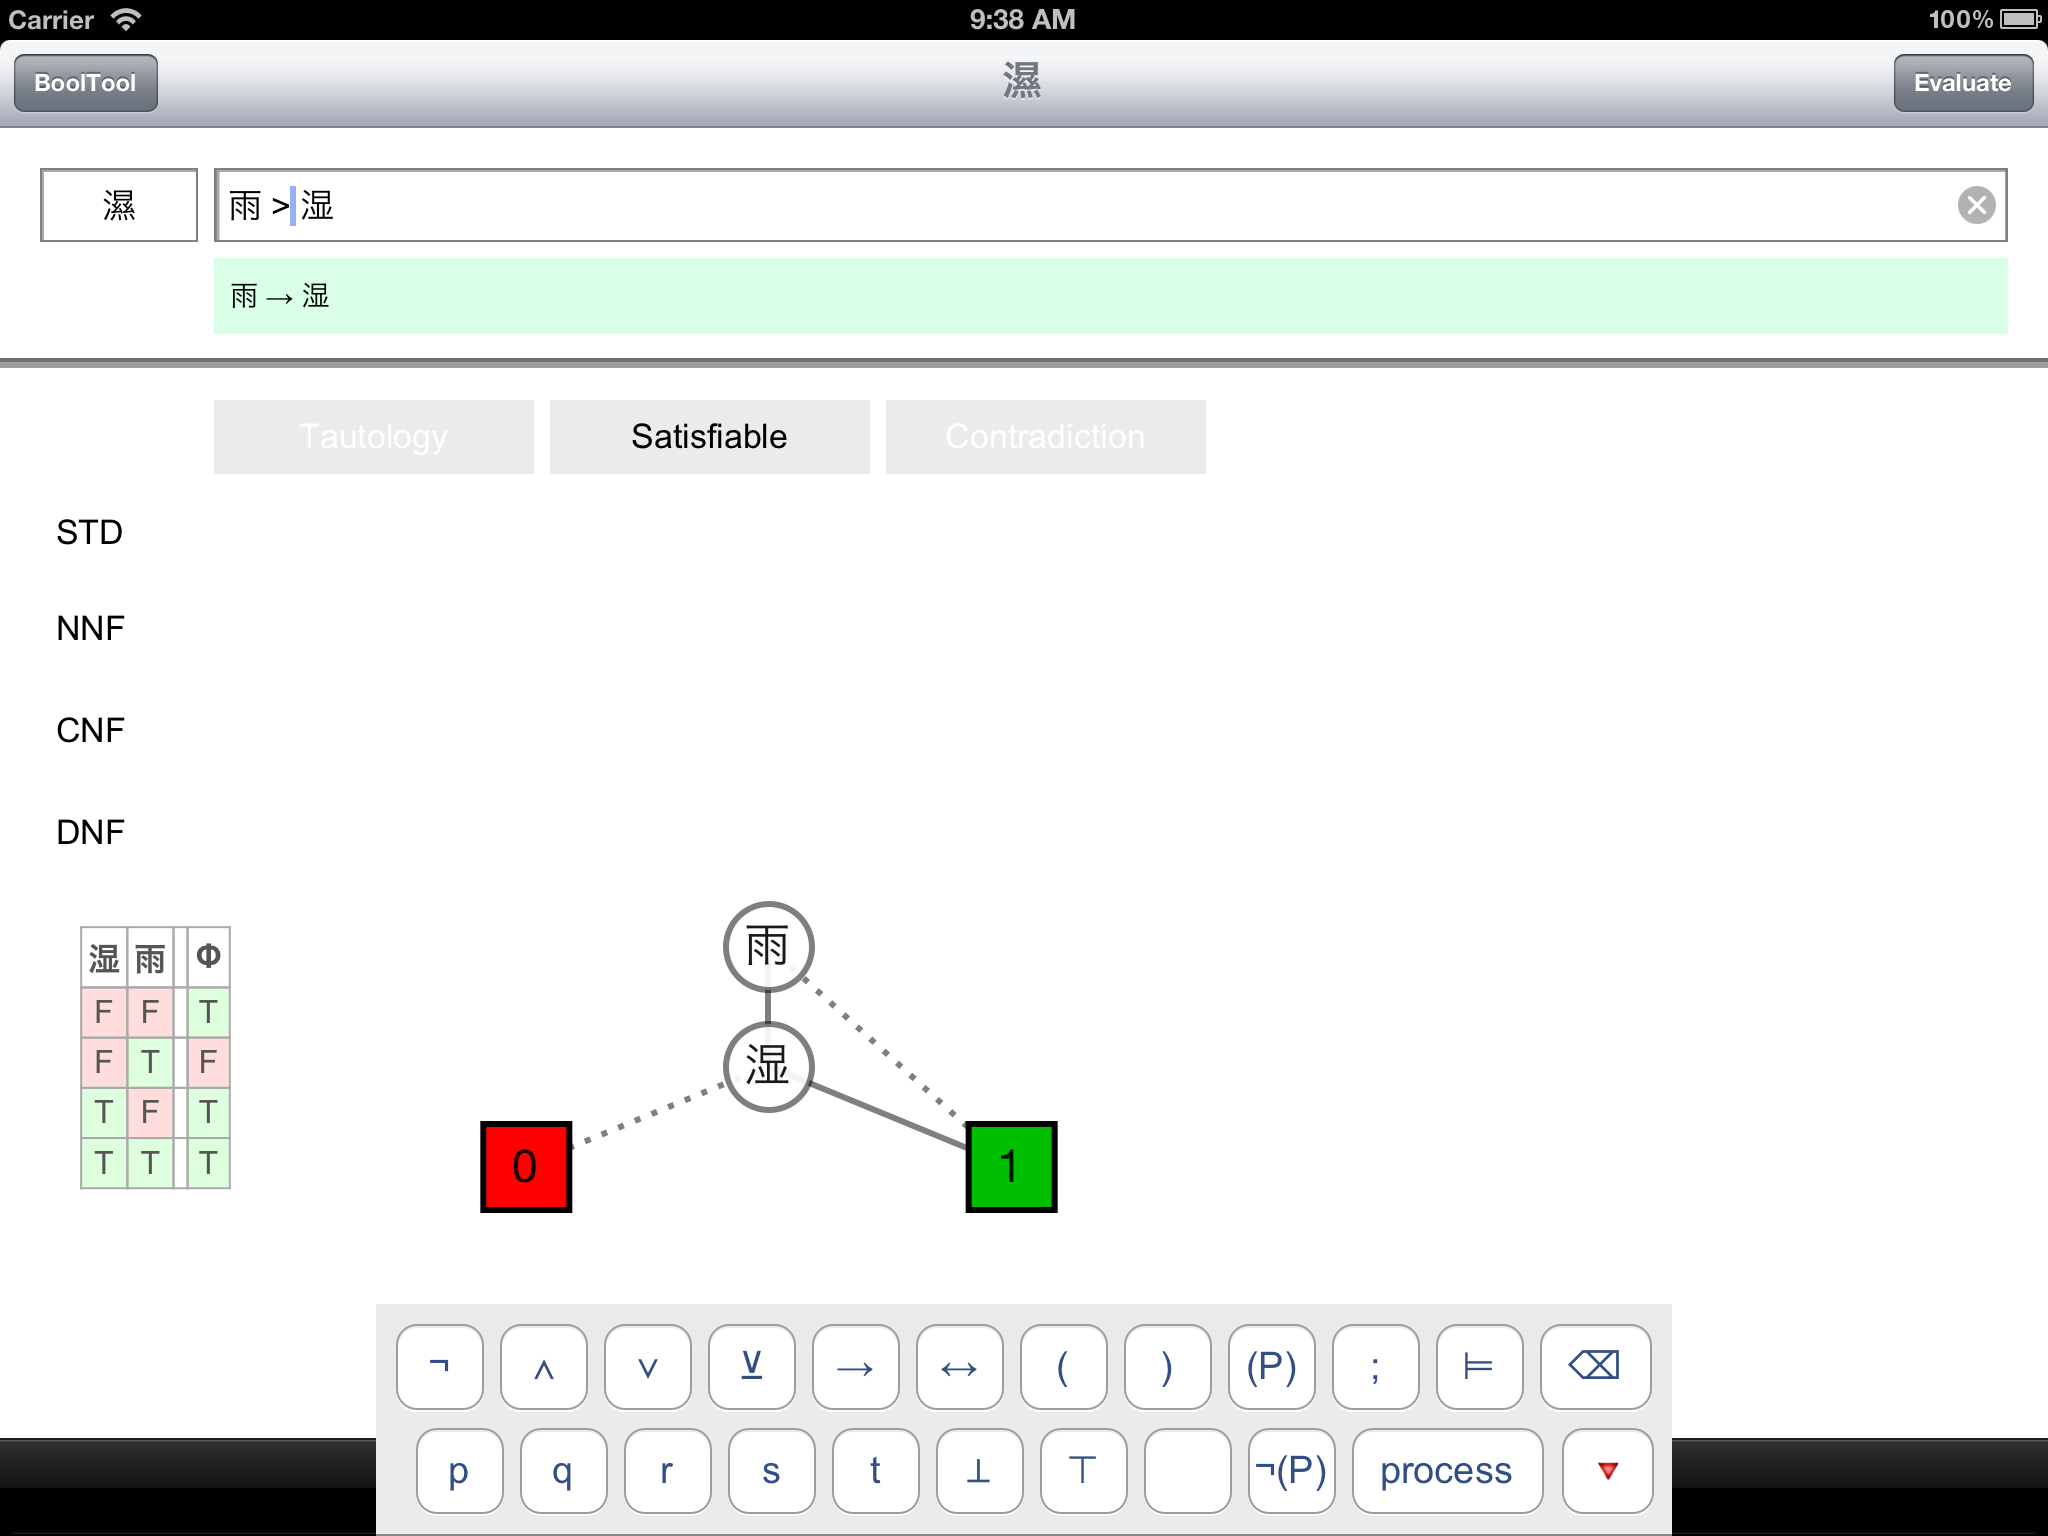
\includegraphics[scale=0.25,trim=16.5cm 11.4cm 34.5cm 31.8cm, clip=true]{concept/RainHD.png}
\caption{Reduced ordered binary decision diagram}
\label{fig:BoolToolROBDD}
\end{center}
\end{figure}

%\begin{figure}[htbp]
%\begin{center}
%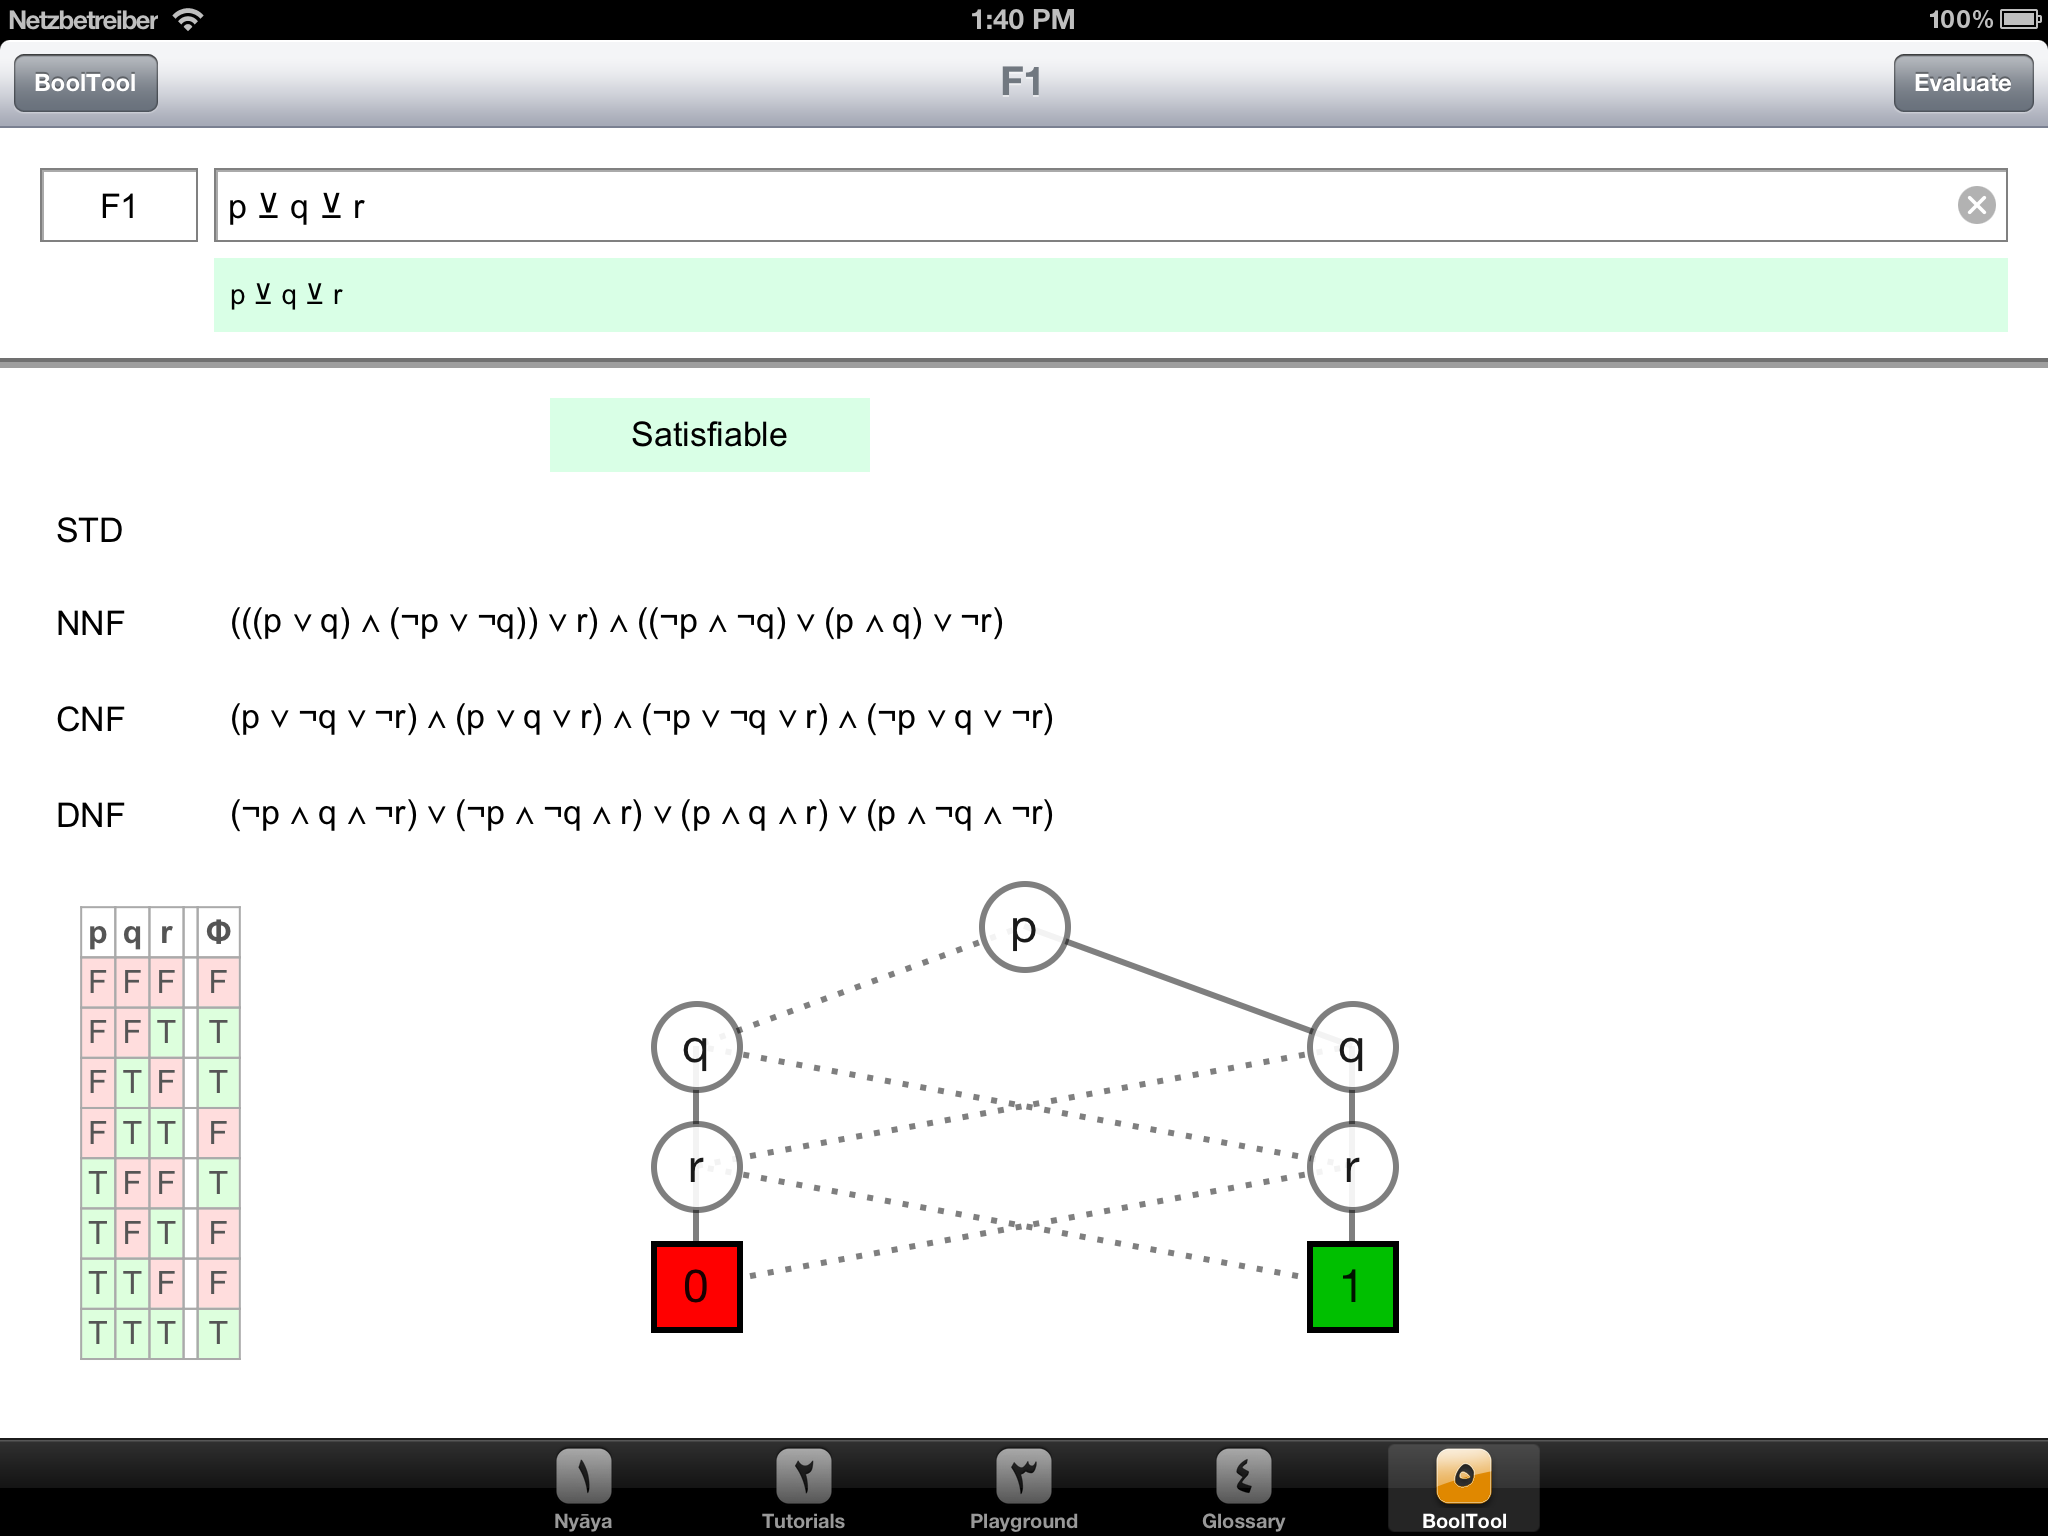
\includegraphics[width=13cm]{concept/BoolTool.png}
%\caption{Boolean function $p \oplus q \oplus r$}
%\label{fig:BoolToolOutput}
%\end{center}
%\end{figure}



